\documentclass[11pt]{article}
    \title{\textbf{Math 217 Homework I}}
    \author{Khac Nguyen Nguyen}
    \date{}
    
    \addtolength{\topmargin}{-3cm}
    \addtolength{\textheight}{3cm}
    
\usepackage{amsmath}
\usepackage{mathtools}
\usepackage{amsthm}
\usepackage{amssymb}
\usepackage{pgfplots}
\usepackage{xfrac}
\usepackage{hyperref}


\usepackage{tikz}
\usetikzlibrary{plotmarks}


\newtheorem{definition}{Definition}[section]
\newtheoremstyle{mystyle}%                % Name
  {}%                                     % Space above
  {}%                                     % Space below
  {\itshape}%                                     % Body font
  {}%                                     % Indent amount
  {\bfseries}%                            % Theorem head font
  {}%                                    % Punctuation after theorem head
  { }%                                    % Space after theorem head, ' ', or \newline
  {\thmname{#1}\thmnumber{ #2}\thmnote{ (#3)}}%                                     % Theorem head spec (can be left empty, meaning `normal')

\theoremstyle{mystyle}
\newtheorem{theorem}{Theorem}[section]
\theoremstyle{definition}
\newtheorem*{exmp}{Example}



\begin{document}
\section*{1.2}
\subsection*{a.}
\begin{align*}
  &g(x) = x^3 - 3x = 0 \\
  \implies & x(x^2-3) = 0 \\
  \implies & x = 0 \text{ or } x = \pm \sqrt{3}
\end{align*}
\begin{align*}
  g'(x) = 3x^2 - 3 
\end{align*}
Thus $g'(0) = -3, g'(\sqrt{3}) = g'(-\sqrt{3}) = 6$ and therefore, $0$ is a sink, $\pm \sqrt{3}$ are sources. \\
\begin{figure}[h] \centering
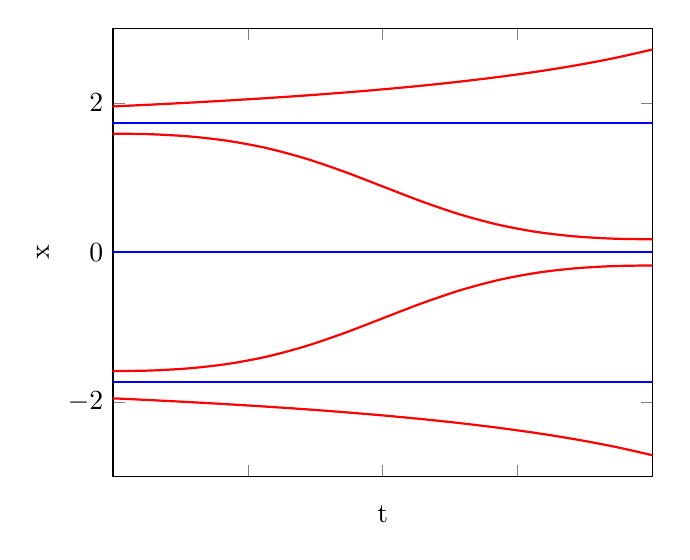
\begin{tikzpicture}
    \begin{axis}[
        view={0}{90},
        domain=-1:1,
        y domain=-3:3,
        xlabel = t,
        ylabel = x,
        xticklabel = \empty,
        xmin=-1, ymin = -3,
        xmax= 1, ymax = 3,
        samples=15
    ]
    \addplot [blue, smooth, thick]{0};
      \addplot [blue, smooth, thick]{sqrt(3)};
      \addplot [blue, smooth, thick]{-sqrt(3)};
      \addplot [red, smooth, thick]{2/(x-2.5)-sqrt(3) + 0.35};
      \addplot [red, smooth, thick]{-2/(x-2.5) + sqrt(3) - 0.35};
      \addplot [red, smooth, thick]{sqrt(2)*x/(x^2+1) + 0.85 - sqrt(3)};
      \addplot [red, smooth, thick]{-sqrt(2)*x/(x^2+1) - 0.85 + sqrt(3)};
    \end{axis}
\end{tikzpicture} 
\end{figure}
\subsection*{b.}
\begin{align*}
  &g(x) = x^4 - x^2 = 0 \\
  \implies & x^2 (x^2-1) = 0 \\
  \implies & x = 0 \text{ or } x = \pm 1
\end{align*}
\begin{align*}
  g'(x) = 4x^3 - 2x
\end{align*}
Thus $g'(0) = 0, g'(1) = 2, g'(-1) = -2$ and therefore, $-1$ is a sink, $1$ is a source and $0$ is neither.
\begin{figure}[h] \centering
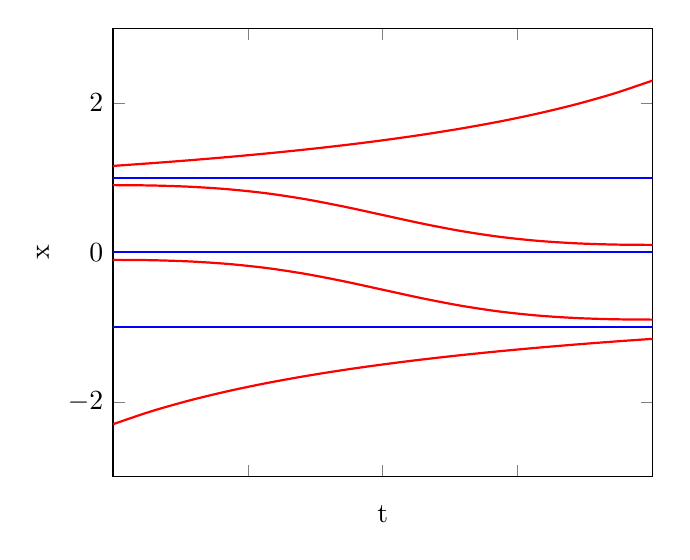
\begin{tikzpicture}
    \begin{axis}[
        view={0}{90},
        domain=-1:1,
        y domain=-3:3,
        xlabel = t,
        ylabel = x,
        xticklabel = \empty,
        xmin=-1, ymin = -3,
        xmax= 1, ymax = 3,
        samples=15
    ]
    \addplot [blue, smooth, thick]{0};
      \addplot [blue, smooth, thick]{1};
      \addplot [blue, smooth, thick]{-1};
      \addplot [red, smooth, thick]{3/(-x-2.5) - 0.3};
      \addplot [red, smooth, thick]{-3/(x-2.5) + 0.3};
      \addplot [red, smooth, thick]{-0.8*x/(x^2+1)+0.5};
      \addplot [red, smooth, thick]{-0.8*x/(x^2+1)-0.5};
    \end{axis}
\end{tikzpicture} 
\end{figure}
\subsection*{c.}
\begin{align*}
  &g(x) = \cos(x) \\
  \implies & x = k\pi + \pi/2 \text{ for } k \in \mathbb{Z}
\end{align*}
\begin{align*}
  g'(x) = -\sin(x) 
\end{align*}
Thus $g'(k\pi + \pi/2) = -1$ for odd $k$, $g'(k\pi + \pi/2) = 1$ for even $k$ and therefore, $k$, $k\pi + \pi/2$ is a sink when $k$ is odd and a source when $k$ is even.  
\begin{figure}[h] \centering
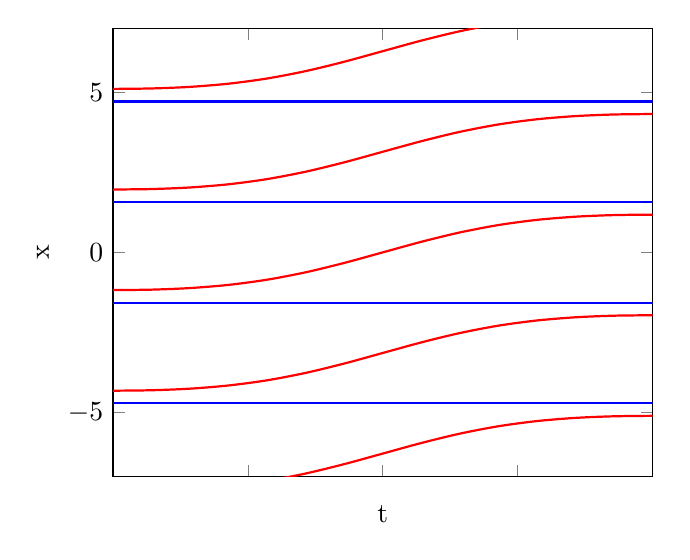
\begin{tikzpicture}
    \begin{axis}[
        view={0}{90},
        domain=-1:1,
        y domain=-7:7,
        xlabel = t,
        ylabel = x,
        xticklabel = \empty,
        xmin=-1, ymin = -7,
        xmax= 1, ymax = 7,
        samples=15
    ]
      \addplot [blue, smooth, thick]{pi/2};
      \addplot [blue, smooth, thick]{3*pi/2};
      \addplot [blue, smooth, thick]{-pi/2};
      \addplot [blue, smooth, thick]{-3*pi/2};
      \addplot [red, smooth, thick]{1.5*pi/2*x/(x^2+1)};
      \addplot [red, smooth, thick]{1.5*pi/2*x/(x^2+1)+2*pi};
      \addplot [red, smooth, thick]{1.5*pi/2*x/(x^2+1)-2*pi};
      \addplot [red, smooth, thick]{1.5*pi/2*x/(x^2+1) + pi};
      \addplot [red, smooth, thick]{1.5*pi/2*x/(x^2+1) - pi};
    \end{axis}
\end{tikzpicture} 
\end{figure}
\pagebreak
\section*{3.}
\subsection*{b.}
\begin{figure}[h]\centering 
    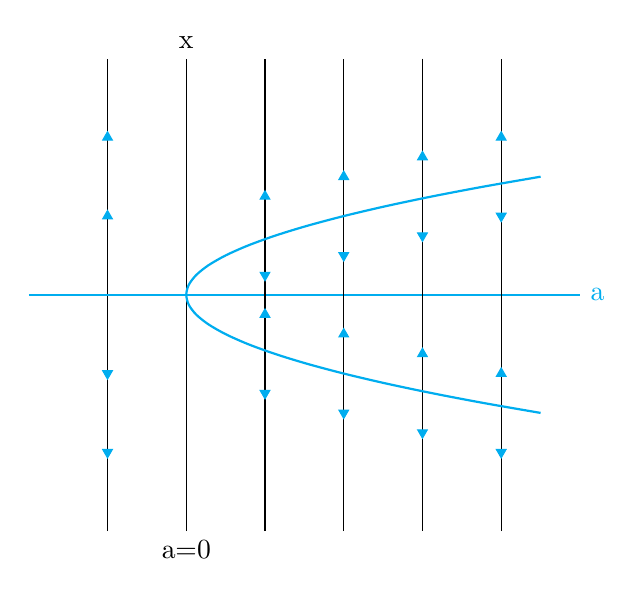
\begin{tikzpicture}
        
        \draw[] (-1, -3) -- (-1, 3) node[above] {};
        \draw[cyan, thick] (-2, -0) -- (5, -0) node[right] {a};
        \draw[] (0, -3) node[below] {a=0}-- (0, 3) node[above] {x};
        \draw[] (1, -3) -- (1, 3) node[above] {};
        \draw[] (2, -3) -- (2, 3) ;
        \draw[] (3, 3) -- (3, -3) node[below] {};
        \draw[] (4, -3) -- (4, 3) node[above] {};

        \draw[scale=0.5, domain=-3:3, smooth, variable=\y,cyan,thick]  plot ({(\y*\y)}, {\y});
        
        %plotmarks
        \node[cyan] at (1,-0.25) {\pgfuseplotmark{triangle*}};
        \node[cyan] at (2,-0.5) {\pgfuseplotmark{triangle*}};
        \node[cyan] at (3,-0.75) {\pgfuseplotmark{triangle*}};
        \node[cyan] at (4,-1) {\pgfuseplotmark{triangle*}};

        \node[cyan,rotate=60] at (1,0.25) {\pgfuseplotmark{triangle*}};
        \node[cyan,rotate=60] at (2,0.5) {\pgfuseplotmark{triangle*}};
        \node[cyan,rotate=60] at (3,0.75) {\pgfuseplotmark{triangle*}};
        \node[cyan,rotate=60] at (4,1) {\pgfuseplotmark{triangle*}};
        
        \node[cyan,rotate=60] at (1,-1.25) {\pgfuseplotmark{triangle*}};
        \node[cyan,rotate=60] at (2,-1.5) {\pgfuseplotmark{triangle*}};
        \node[cyan,rotate=60] at (3,-1.75) {\pgfuseplotmark{triangle*}};
        \node[cyan,rotate=60] at (4,-2) {\pgfuseplotmark{triangle*}};
        
        \node[cyan] at (1,1.25) {\pgfuseplotmark{triangle*}};
        \node[cyan] at (2,1.5) {\pgfuseplotmark{triangle*}};
        \node[cyan] at (3,1.75) {\pgfuseplotmark{triangle*}};
        \node[cyan] at (4,2) {\pgfuseplotmark{triangle*}};
        
        \node[cyan] at (-1,1) {\pgfuseplotmark{triangle*}};
        \node[cyan] at (-1,2) {\pgfuseplotmark{triangle*}};
        \node[cyan,rotate=60] at (-1,-1) {\pgfuseplotmark{triangle*}};
        \node[cyan,rotate=60] at (-1,-2) {\pgfuseplotmark{triangle*}};
    \end{tikzpicture}
\end{figure}
\subsection*{c.}
\begin{figure}[h]\centering 
    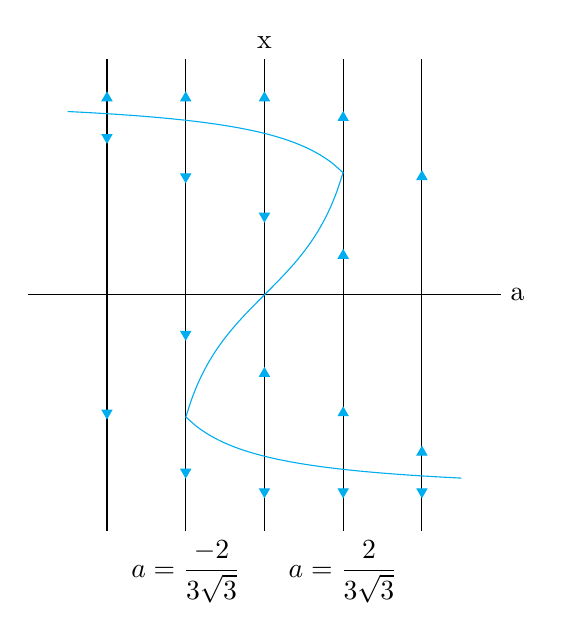
\begin{tikzpicture}
        
        \draw[] (-2, -3) -- (-2, 3) node[above] {};
        \draw[] (-3, -0) -- (3, 0) node[right] {a}; 
        \draw[] (-1, -3) node[below] {$a = \displaystyle\frac{-2}{3\sqrt{3}}$} -- (-1, 3) node[above] {};
        \draw[] (0, -3) -- (0, 3) node[above] {x};
        \draw[] (1, -3) node[below] {$a = \displaystyle\frac{2}{3\sqrt{3}}$} -- (1, 3) node[above] {};
        \draw[] (2, -3) -- (2, 3) ;  
        \draw[scale=1, domain=-1:1, smooth, variable=\x, cyan] plot ({\x}, {tan(deg(\x))});
        \draw[scale=1, domain=-1:2.5, smooth, variable=\x, cyan] plot ({\x}, {1 / (\x+2) - 2.55});
        \draw[scale=1, domain=-2.5:1, smooth, variable=\x, cyan] plot ({\x}, {-1 / (-\x+2) + 2.55});
        %plotmarks
        \node[cyan] at (0,-1) {\pgfuseplotmark{triangle*}};
        \node[cyan] at (1,0.5) {\pgfuseplotmark{triangle*}};
        \node[cyan] at (2,1.5) {\pgfuseplotmark{triangle*}};
        \node[cyan] at (2,-2) {\pgfuseplotmark{triangle*}};
        \node[cyan] at (1,-1.5) {\pgfuseplotmark{triangle*}};
        \node[cyan] at (-2,2.5) {\pgfuseplotmark{triangle*}};
        \node[cyan] at (-1,2.5) {\pgfuseplotmark{triangle*}};
        \node[cyan] at (0,2.5) {\pgfuseplotmark{triangle*}};
        \node[cyan] at (1,2.25) {\pgfuseplotmark{triangle*}};

        \node[cyan,rotate=60] at (0,1) {\pgfuseplotmark{triangle*}};
        \node[cyan,rotate=60] at (-1,-0.5) {\pgfuseplotmark{triangle*}};
        \node[cyan,rotate=60] at (-2,-1.5) {\pgfuseplotmark{triangle*}};
        \node[cyan,rotate=60] at (-2,2) {\pgfuseplotmark{triangle*}};
        \node[cyan,rotate=60] at (-1,1.5) {\pgfuseplotmark{triangle*}};
        \node[cyan,rotate=60] at (2,-2.5) {\pgfuseplotmark{triangle*}};
        \node[cyan,rotate=60] at (1,-2.5) {\pgfuseplotmark{triangle*}};
        \node[cyan,rotate=60] at (0,-2.5) {\pgfuseplotmark{triangle*}};
        \node[cyan,rotate=60] at (-1,-2.25) {\pgfuseplotmark{triangle*}};
    \end{tikzpicture}
\end{figure}
\pagebreak
\section*{5.}
\subsection*{a.}
\begin{figure}[h] \centering
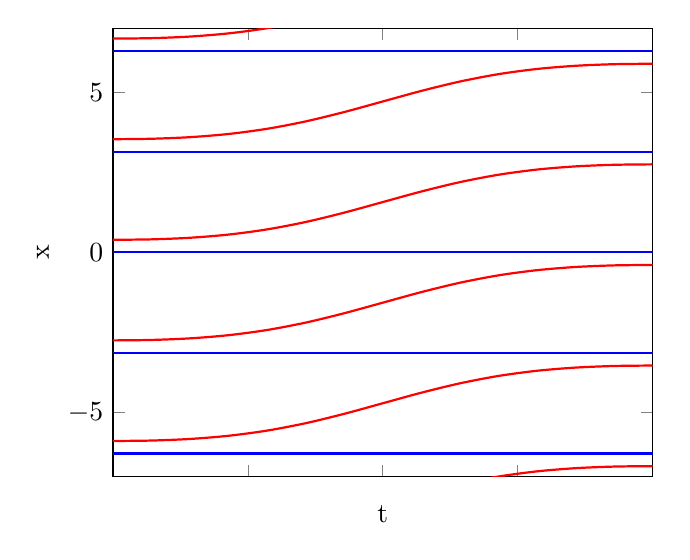
\begin{tikzpicture}
    \begin{axis}[
        view={0}{90},
        domain=-1:1,
        y domain=-7:7,
        xlabel = t,
        ylabel = x,
        xticklabel = \empty,
        xmin=-1, ymin = -7,
        xmax= 1, ymax = 7,
        samples=15
    ]
      \addplot [blue, smooth, thick]{0};
      \addplot [blue, smooth, thick]{pi};
      \addplot [blue, smooth, thick]{-pi};
      \addplot [blue, smooth, thick]{2*pi};
      \addplot [blue, smooth, thick]{-2*pi};
      \addplot [red, smooth, thick]{1.5*pi/2*x/(x^2+1) + pi/2};
      \addplot [red, smooth, thick]{1.5*pi/2*x/(x^2+1)+2*pi +pi/2};
      \addplot [red, smooth, thick]{1.5*pi/2*x/(x^2+1)-2*pi + pi/2};
      \addplot [red, smooth, thick]{1.5*pi/2*x/(x^2+1) + pi+ pi/2};
      \addplot [red, smooth, thick]{1.5*pi/2*x/(x^2+1) - pi/2};
      \addplot [red, smooth, thick]{1.5*pi/2*x/(x^2+1) - 5*pi/2};
    \end{axis}
\end{tikzpicture}
\end{figure}
\subsection*{b.}
We want to look at the zeros of $ax - \sin(x)$, or the intersection between $y = -ax$ and $y = \sin(x)$. we notice that 
\begin{itemize}
  \item $x=0$ is always an intersection
  \item At $a = 1, -1$ there is no other intersection. 
  \item As $|a|$ approaches 0, the slope of the line decrease thus there is more intersection. 
  \item At $a = 0$, there is infinitely many intersections.
\end{itemize}
\subsection*{c.}
\begin{figure}[h]\centering 
    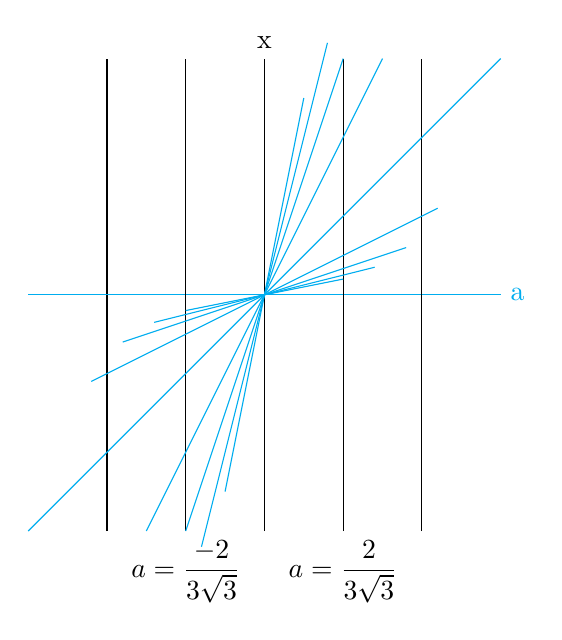
\begin{tikzpicture} 
        \draw[] (-2, -3) -- (-2, 3) node[above] {};
        \draw[cyan] (-3, -0) -- (3, 0) node[right] {a}; 
        \draw[] (-1, -3) node[below] {$a = \displaystyle\frac{-2}{3\sqrt{3}}$} -- (-1, 3) node[above] {};
        \draw[] (0, -3) -- (0, 3) node[above] {x};
        \draw[] (1, -3) node[below] {$a = \displaystyle\frac{2}{3\sqrt{3}}$} -- (1, 3) node[above] {};
        \draw[] (2, -3) -- (2, 3) ;  
        \draw[scale=1, domain=-1:1, smooth, variable=\x, cyan] plot ({\x}, {\x/5});
        \draw[scale=1, domain=-1.4:1.4, smooth, variable=\x, cyan] plot ({\x}, {\x/4});
        \draw[scale=1, domain=-1.8:1.8, smooth, variable=\x, cyan] plot ({\x}, {\x/3});
        \draw[scale=1, domain=-2.2:2.2, smooth, variable=\x, cyan] plot ({\x}, {\x/2});
        \draw[scale=1, domain=-3:3, smooth, variable=\x, cyan] plot ({\x}, {\x});
        \draw[scale=1, domain=-1.5:1.5, smooth, variable=\x, cyan] plot ({\x}, {2*\x});
        \draw[scale=1, domain=-1:1, smooth, variable=\x, cyan] plot ({\x}, {3*\x});
        \draw[scale=1, domain=-0.8:0.8, smooth, variable=\x, cyan] plot ({\x}, {4*\x});
        \draw[scale=1, domain=-0.5:0.5, smooth, variable=\x, cyan] plot ({\x}, {5*\x});
        %plotmarks

    \end{tikzpicture}
\end{figure}
\newpage
The blue line have more intersection with the line $a = b$ as $b \to 0$ and less intersection until there is only 1 as $|b| \to \infty$. On each line $a = b$, we can write a partition of where the points of the partition are the intersections of $a=b$ with the blue line. The arrow will alternate on such interval. At $x = 0$, the derivative of $\sin(x) + ax$ have the same sign as $a$ which will indicate the direction of the arrow at the intervals furthest from 0. \\
Note: the blue "line" should not be exactly line. 
\pagebreak
\section*{11.}
\subsection*{a.}
\begin{align*}
  &x' = x^2 \\
  \implies & \displaystyle\frac{dx}{dt} = x^2 \\
  \implies & \int \displaystyle\frac{dx}{x^2} = \int dt \\
  \implies & -\displaystyle\frac{1}{3x^3} = t + C \\
  \implies &x(t) = \sqrt[3]{\displaystyle\frac{-1}{3 (t+C)}}
\end{align*}
\subsection*{b.}
For each $C \in \mathbb{R}$, the domain of $t$ is $\mathbb{R} \backslash \{-C\}$
and the domain of $x$ is $\mathbb{R} \backslash \{0\}$. 
\subsection*{c.}
Consider $x(t) = \tan(\pi t /2)$, then $x$ is defined on $(-1,1)$ but not on $[-1,1)$ or $(-1,1]$. We also have that $x(0) = 0$. The differential equation is then 
\[
  x' = \displaystyle\frac{\pi}{2} (1 + \tan^2(\pi t /2)) = \displaystyle\frac{\pi}{2} (1 + x^2)
\]
\pagebreak
\section*{12.}
\subsection*{a.}
\begin{align*}
  &x' = x^{1/3} \\
  \implies & \int \displaystyle\frac{dx}{x^{1/3}} = \int dt \\
  \implies & \displaystyle\frac{3}{2}x^{2/3} = t + C \\
  \implies & x = 
  \begin{cases}
    \displaystyle\frac{2}{3}\left(t+C \right)^{3/2}, &\text{ if } t > -C \\
    0, &\text{ if } t < -C
  \end{cases}
\end{align*}
since $x'(-C) = 0$. Hence, for any $-C>0$ or $C < 0$, $x(t) =  0$. 
\subsection*{b.}
\begin{align*}
  &x' = x /t \\
  \implies & \int \displaystyle\frac{dx}{x} = \int \displaystyle\frac{dt}{t} \\
  \implies & \ln(x) = \ln(t) + C \\
  \implies & x = e^{\ln(t) + C} = te^C = tC'
\end{align*}
$x(0) = 0$ regardless of $C'$ thus every solution in the family satisfy the initial condition.
\subsection*{c.}
\begin{align*}
  &x' = x /t^2 \\
  \implies & \int \displaystyle\frac{dx}{x} = \int \displaystyle\frac{dt}{t^2} \\
  \implies & \ln(x) = \frac{-1}{t} + C \\
  \implies & x = e^{\frac{-1}{t} + C} = e^{-1/t} e^C = C' e^{-1/t}
\end{align*}
Since $t\ne 0$ from $x' = \displaystyle\frac{x}{t^2}$, and $x$ is discontinuous at $0$ regardless of $x(0)$:
\[
  \lim_{t\to 0^+} x(t) = 0 \ne \infty \lim_{t \to 0^-} x(t)
\]
There is no continuous solution.  
\pagebreak
\section*{2.2}
\subsection*{a.}
We first find the eigenvalue 
\[
  \begin{vmatrix}
    1 - \lambda & 2 \\
    0 & 3 - \lambda
  \end{vmatrix}
  = 0 \implies \lambda \in \{1,3\} 
\]
For $\lambda = 1$, 
\[
  \begin{pmatrix}
    0 & 2 \\
    0 & 2
  \end{pmatrix}
  v
  = 0 \implies
  v = 
  \begin{pmatrix}
    1 \\
    0
  \end{pmatrix}
\]
For $\lambda = 3$, 
\[
  \begin{pmatrix}
    -2 & 2 \\
    0 & 0
  \end{pmatrix}
  v
  = 0 \implies
  v = 
  \begin{pmatrix}
    1 \\
    1
  \end{pmatrix}
\]
Thus, 
\[
  X = C_1e^t 
  \begin{pmatrix}
    1 \\
    0
  \end{pmatrix}
  + C_2e^{3t} 
  \begin{pmatrix}
    1 \\
    1
  \end{pmatrix}
\]
\subsection*{b.}
We first find the eigenvalue 
\[
  \begin{vmatrix}
    1 - \lambda & 2 \\
    3 & 6 - \lambda
  \end{vmatrix}
  = 0 \implies \lambda \in \{0,7\} 
\]
For $\lambda = 0$, 
\[
  \begin{pmatrix}
    1 & 2 \\
    3 & 6
  \end{pmatrix}
  v
  = 0 \implies
  v = 
  \begin{pmatrix}
    -2 \\
    1
  \end{pmatrix}
\]
For $\lambda = 7$, 
\[
  \begin{pmatrix}
    -6 & 2 \\
    3 & -1
  \end{pmatrix}
  v
  = 0 \implies
  v = 
  \begin{pmatrix}
    1 \\
    3
  \end{pmatrix}
\]
Thus, 
\[
  X = C_1 
  \begin{pmatrix}
    -2 \\
    1
  \end{pmatrix}
  + 
  C_2 e^{7t} 
  \begin{pmatrix}
    1 \\
    3
  \end{pmatrix}
\]
\subsection*{c.}
We first find the eigenvalue 
\[
  \begin{vmatrix}
    1 -\lambda & 2 \\
    1 & 0 - \lambda
  \end{vmatrix}
  = 0 \implies \lambda \in \{-1,2\} 
\]
For $\lambda = -1$, 
\[
  \begin{pmatrix}
    2 & 2 \\
    1 & 1
  \end{pmatrix}
  v
  = 0 \implies
  v = 
  \begin{pmatrix}
    1 \\
    0
  \end{pmatrix}
\]
For $\lambda = 2$, 
\[
  \begin{pmatrix}
    -1 & 2 \\
    1 & -2
  \end{pmatrix}
  v
  = 0 \implies
  v = 
  \begin{pmatrix}
    2 \\
    1
  \end{pmatrix}
\]
Thus, 
\[
  X = C_1 e^{-t} 
  \begin{pmatrix}
    1 \\
    0
  \end{pmatrix}
  + 
  C_2 e^{2t} 
  \begin{pmatrix}
    2 \\
    1
  \end{pmatrix}
\]
\subsection*{d.}
We first find the eigenvalue 
\[
  \begin{vmatrix}
    1 - \lambda & 2 \\
    3 & -3 - \lambda
  \end{vmatrix}
  = 0 \implies \lambda = - 1 \pm \sqrt{10} 
\]
For $\lambda = -1 + \sqrt{10}$, 
\[
  \begin{pmatrix}
    2 - \sqrt{10} & 2 \\
    3 & -2 - \sqrt{10}
  \end{pmatrix}
  v
  = 0 \implies
  v = 
  \begin{pmatrix}
    2 + \sqrt{10} \\
    3
  \end{pmatrix}
\]
For $\lambda = -1 - \sqrt{10}$, 
\[
  \begin{pmatrix}
    2 + \sqrt{10} & 2 \\
    3 & -2 + \sqrt{10}
  \end{pmatrix}
  v
  = 0 \implies
  v = 
  \begin{pmatrix}
    2 - \sqrt{10} \\
    3
  \end{pmatrix}
\]
Thus, 
\[
  X = C_1e^{-1 + \sqrt{10}} 
  \begin{pmatrix}
    2 + \sqrt{10} \\
    3
  \end{pmatrix}
  + C_2 e^{-1 - \sqrt{10}} 
  \begin{pmatrix}
    2 - \sqrt{10} \\
    3
  \end{pmatrix}
\]
\pagebreak
\section*{2.3}

\begin{itemize}
  \item figure 1: c \\
  \item figure 2: b \\
  \item figure 3: d \\
  \item figure 4: a
\end{itemize}
\pagebreak
\section*{2.6}
The characteristic equation is $r^2 + br + k = 0$ thus for the system to have real and distinct eigenvalue, we need $b^2 -4k > 0$ thus $b > 2k$ (assuming constant $b \ge 0, k > 0$) and the general solution should be 
\[
  x(t) = C_1 e^{r_1 t} + C_2 e^{r_2 t}
\]
where $r_1, r_2$ are the respective solution of the characteristic equation, that is 
\[
  r_{1,2} = \displaystyle\frac{-b \pm \sqrt{b^2-4k}}{2} 
\]
We have $x(0) = 1$ thus $C_1 + C_2 = 1$. Also, $b,k>0$, $r_{1,2} < 0$ and thus it is a damped harmonic oscillator. 
\pagebreak
\section*{2.8}
Let the matrix be 
\[
  \begin{pmatrix}
    a & b \\
    c & d
  \end{pmatrix}
\]
If $b = 0$ or $c=0$ then $(a,d) \in \{(1,0), (0,1)\}$.
Otherwise, the eigenvalue is the solution of 
\[
  (a - \lambda)(d-\lambda) - bc = \lambda^2 - \lambda(a + d) + (ad-bc) = 0 
\]
Thus we have the system of equation 
\[
  \begin{cases}
    ad - bc = 0 \\
    1 - (a+d) + ad - bc = 0
  \end{cases}
\]
Thus, 
\[
  ad = bc \text{ and } a + d = 1
\]
and the matrix can be rewritten as  
\[
  \begin{pmatrix}
    a & b \\
    a(1-a)/b & 1-a
  \end{pmatrix}
\]
\pagebreak
\section*{2.14}
Suppose $\lambda_1, \lambda_2$ are eigenvalues of a 2 by 2 matrix with non-linearly dependent eigenvectors. That is 
$\lambda_1 \ne \lambda_2$ and $v_1 = x v_2$ for some $x \in \mathbb{R}$. Then we have 
\[
  x \lambda_2 v_2 =  x A v_2 = Ax v_2 = A v_1 = \lambda_1 v_1 = \lambda_1 x v_2 
\]
which means that $\lambda_2 = \lambda_1$ are not distinct. \\
Therefore, the eigenvectors of a 2 × 2 matrix corresponding to distinct real eigenvalues are always linearly independent.
\end{document}

